\chapter{Überblick und Entwurf}
\label{cha_overview}

Das Ziel dieser Arbeit ist es, ein System zu entwickeln, das mithilfe von Pseudonymisierung die datenschutzgerechte Speicherung von Überwachungsdaten ermöglicht, wobei die Identität eines Pseudonymhalters im Bedarfsfall durch die Kollaboration verschiedener Akteure unter Nutzung eines kryptographischen Schwellwertschemas aufdeckbar sein muss. Um eine Basis für die Erarbeitung von Anforderungen und für einen Systementwurfs zu erhalten, soll nun kurz dargelegt werden, wie die verschiedenen Verfahren ineinander greifen. 

Aus Datenquellen wie Firewalls, Zugriffsprotokollen von Dateisystemen oder auch elektronischen Türschlössern werden personenbeziehbare Logdaten\footnote{
  Da im Bereich technischer Systeme eher von Logdaten oder Protokolldaten im Gegensatz zu Überwachungsdaten gesprochen wird, wird diese Terminologie hier verwendet. Im Rahmen dieser Arbeit sind die Begriffe jedoch synonym zu verstehen.
} an ein SIEM-System gesendet und dort gespeichert.\\
In diesen Datenfluss wird nun durch ein zu entwickelndes System eingegriffen, das die personenbeziehbaren Informationen des Logdatums\footnote{
  Um Missverständnisse auszuschließen, sei darauf hingewiesen, dass das Wort Datum in dieser Arbeit als Beschreibung einer Informationseinheit und nicht eines Zeitpunkts verwendet wird. 
} durch ein Pseudonym ersetzt. Die Zuordnung zwischen dem gesetzten Pseudonym und der personenbeziehbaren Information wird durch ein kryptographisches Schwellwertschema verschlüsselt und in dem System gespeichert.

Damit die anschließend auf den pseudonymisierten Logdaten stattfindende Anomalieerkennung Aktionen eines Mitarbeiters verknüpfen kann, muss sichergestellt werden, dass für einen speziellen Benutzer das gleiche Pseudonym verwendet wird. Wird nun durch die Anomalieerkennung ein Angriff erkannt, so können berechtigte Benutzer durch kooperative Entschlüsselung der Pseudonymzuordnung den hinter dem Pseudonym stehenden Benutzer wieder aufdecken.

\begin{figure}[]
    \centering
        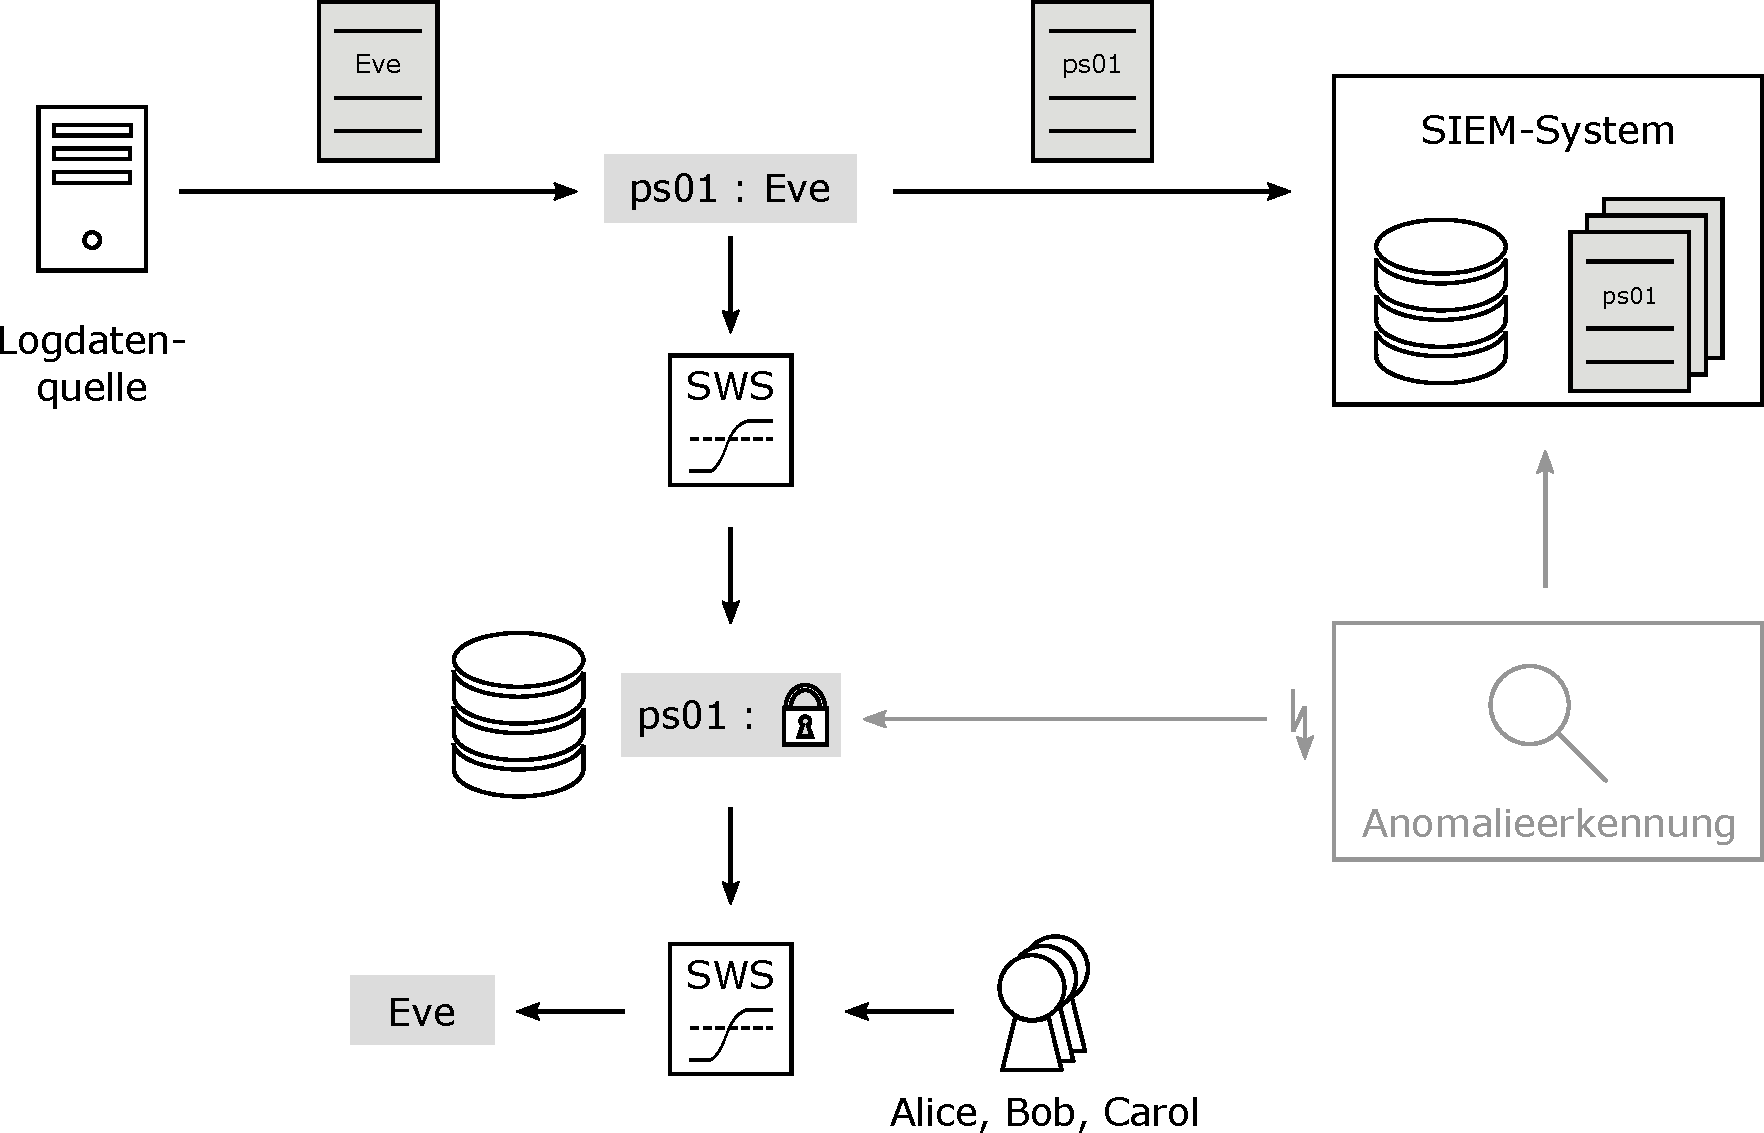
\includegraphics[width=0.9\textwidth]{dia/overview.pdf}
    \caption{Übersicht zu dem angestrebten Verfahren.}
    \label{fig:overview_initial}
\end{figure}

Anschaulich wird der Vorgang in Abbildung \ref{fig:overview_initial} dargestellt: Die Benutzerin \textit{Eve} agiert in dem Unternehmensnetzwerk. Ihre Aktionen werden protokolliert und Logdaten, die ihren Benutzernamen enthalten, werden versendet. Dieser Benutzername wird durch das Pseudonym \textit{ps01} ersetzt. Die Zuordnung des Pseudonyms wird nun mithilfe eines kryptographischen Schwellwertschemas verschlüsselt und in einer Datenbank abgelegt. Das pseudonymisierte Logdatum wird im SIEM-System gespeichert.\\
Eingesetzte Anomalieerkennungsverfahren können anschließend auf die Daten des SIEM-Systems zugreifen. Wird ein möglicher Insider-Angriff durch einen Benutzer mit dem Pseudonym \textit{ps01} erkannt, so kann die Zuordnung zu dem ursprünglichen Benutzernamen mithilfe des Schwellwertschemas wieder aufgedeckt werden. Hierzu ist jedoch die Mitarbeit von \textit{Alice}, \textit{Bob} und \textit{Carol} notwendig, die jeweils im Besitz eines Teils des Entschlüsselungsschlüssels sind. Stimmen sie der Aufdeckung zu, so wird \textit{Eve} als Halter des Pseudonyms \textit{ps01} und damit als möglicher Innentäter aufgedeckt.

In diesem Kapitel werden zentrale Anforderungen an ein solches System entwickelt und eine abstrakte Architektur für ein solches entworfen. Anschließend wird darauf aufbauend ein Angreifermodell für das System definiert.

\section{Anforderungen}

\label{sec_impl_requirements}

Neben den primären Anforderungen, die sich direkt aus der Funktionsbeschreibung des Systems und dem Zusammenspiel der enthaltenen Verfahren ergeben, sollte das System noch weitere Eigenschaften wie beispielsweise die Erweiterbarkeit um zusätzliche Datenschutztechniken erfüllen. All diese Anforderungen sollen im folgenden Abschnitt aufgestellt und näher erläutert werden.

\subsection{Integration in das SIEM-System}

\label{subsec_impl_requirements_ossimintegration}

Für den Eingriff in den Datenfluss der Logdaten zwischen ihrer Quelle und dem verwendeten SIEM-System muss eine geeignete Stelle gefunden werden. Hierzu müssen Auswirkungen des Eingriffs betrachtet sowie die Vor- bzw. Nachteile der verschiedenen Möglichkeiten gegeneinander abgewogen werden. 

\subsection{Pseudonymisierung}

\label{subsec_impl_requirements_pseudonymity}

%- Lang genug für geringe Kollisionswsk.
%- Eindeutig
%- Durchsuchbar (mim Hinblick auf threshold)
%- Anwendungsfallabhängige Parameter für Nutzzeit, ... (Rückblick auf Kapitel 3)

Die Pseudonymisierung muss es ermöglichen, nach Aufdecken eines Eintrags wieder auf den ursprünglichen Dateninhalt schließen zu können. Daher müssen die Pseudonyme für die Zeit ihrer Speicherung eindeutig sein, d.h. es darf zu keiner Mehrfachverwendung von Pseudonymen kommen. 

Weiterhin muss es beim Pseudonymisieren von Logeinträgen eine Möglichkeit geben, zu überprüfen, ob für ein Datum bereits ein Pseudonym vergeben wurde. So kann sichergestellt werden, dass in einem bestimmten Zeitraum Logeinträge zu einer Person stets mit dem gleichen Pseudonym versehen werden, um mithilfe der Verknüpfung von Einträgen Anomalieerkennungsverfahren sinnvoll einsetzen zu können. Auf diese Anforderung wird in Abschnitt \ref{sec_state_se} noch genauer eingegangen.

Außerdem muss es eine Möglichkeit geben, die Parameter der Pseudonymisierung, wie den Zeitraum ihrer Verwendung, konfigurierbar zu machen (siehe Abschnitt \ref{sec_state_pseudonymity}).

\subsection{Einsatz eines kryptographischen Schwellwertschemas}

\label{subsec_impl_requirements_threshold}

%- Verteiltes Modell 
%- Kommunikation
%- Schlüsselmanagement
%- ...

Der Einsatz eines kryptographischen Schwellwertschemas setzt eine verteilte Anwendung voraus, die den Zugriff für die Pseudonymisierungskomponente sowie für die bei der Entschlüsselung eines Eintrags beteiligten Akteure bereitstellt. Die für das Schwellwertschema nötigen, in Abschnitt \ref{sec_basics_threshold} beschriebenen Parameter \(t\) und \(n\) und auch die beteiligten Share-Besitzer müssen in dem System initial konfigurierbar sein.

In der Phase der Schlüsselgenerierung muss das System die Kommunikation und Koordination aller Beteiligten unterstützen. Die hier erstellten Schlüssel und \textit{Shares} müssen an geeigneten Stellen sicher gespeichert und abrufbar sein. Für diese Phase gibt es zwei Möglichkeiten:
\begin{itemize}
  \item \textbf{Zentrale Generierung von öffentlichem Schlüssel und Shares}: Eine vertrauenswürdige Komponente generiert ein Schlüsselpaar und zerlegt den geheimen Schlüssel in die einzelnen Shares, die anschließend verteilt werden können. 
  \item \textbf{Verteilte Schlüsselgenerierung}: Hierbei generieren die einzelnen Share-Besitzer jeweils ihre eigenen Shares. Durch verteilte Berechnungen kann hieraus der gemeinsame öffentliche Schlüssel erzeugt werden. Der geheime Schlüssel liegt auf diese Weise niemals an einer Stelle vor und ein vertrauenswürdiger Dritter ist nicht notwendig. Aus diesem Grund ist diese Lösung zu bevorzugen.
\end{itemize}

Der für die Verschlüsselung erforderliche öffentliche Schlüssel muss so vorliegen, dass er bei der Verschlüsselung eines Pseudonym-Datensatzes genutzt werden kann.

Bei der Entschlüsselung eines Eintrags, also der Aufdeckung eines Pseudonyms, muss das System wiederum die beteiligten Akteure koordinieren. Anschließend muss eine Komponente die Rolle des \textit{Combiners} übernehmen, so dass anschließend der den Pseudonymhalter beschreibende, entschlüsselte Datensatz im System  vorliegt.

\subsection{Benutzerinteraktion}

\label{subsec_impl_requirements_userinteraction}

%- Proxy: Konfiguration der Plugins

%- Pseudo-App: Statusanzeige angemeldeter Benutzer(Admin), Initialisierung der Schlüsselgenerierung nach Nutzerauswahl(Admin), Anlegen von Aufdeckanfragen, Statusanzeige von Aufdeckanfragen, Systemstatus

%- Einzelne Teilnehmer sollten Client-Anwendungen besitzen, um auf Anfragen reagieren zu können (Generation eigener Schlüssel, gemeinsame Schlüsselgenerierung, ... ) Konsolenanwendung? 

Die zu entwickelnde verteilte Anwendung wird an verschiedenen Stellen Benutzerinteraktion erfordern.

Das Konfigurieren des Systems zur Integration verschiedener Datenquellen muss einem berechtigten Nutzer zugänglich gemacht werden. Ebenso sollte es für die -- in der Aufgabenstellung geforderte -- Erweiterbarkeit um weitere Datenschutztechniken relativ leicht sein, diese Techniken im System nutzen zu können. 

Für pseudonymisierte Datensätze muss es berechtigten Benutzern ermöglicht werden, Anfragen zur Aufdeckung eines Pseudonyms zu stellen und sich über ihren Status informiert zu halten.

Einem Administrator des Systems sollte es für die Benutzung eines kryptographischen Schwellwertschemas ermöglicht werden, grundlegende Parameter des Systems wie die Schwellwertparameter und die beteiligten Nutzer auszuwählen sowie die Initialisierung des Schemas anzustoßen. 

Die am Schwellwertschema beteiligten Nutzer müssen die Möglichkeit erhalten, eine Übersicht über sie betreffende Anfragen zur Aufdeckung eines Pseudonym-Datensatzes zu bekommen sowie einzelne Anfragen abzulehnen oder sich am Prozess des Aufdeckens mithilfe des Schwellwertschemas zu beteiligen. 

\subsection{Erweiterbarkeit um neue Datenquellen}

\label{subsec_impl_requirements_differentsources}

Das umzusetzende System sollte es ermöglichen, Daten aus verschiedenen Quellen und (abhängig vom gewählten Eingriffspunkt in OSSIM) auch in verschiedenen Formaten entgegenzunehmen und mithilfe der umgesetzten Datenschutztechniken verändern zu können. Dabei muss das Format der Logdaten grundsätzlich beibehalten werden, um die Behandlung der Daten in dem verwendeten SIEM-System weiterhin zu ermöglichen.

\subsection{Erweiterbarkeit um neue Datenschutztechniken}

\label{subsec_impl_requirements_plugins}

Neben der im Fokus dieser Arbeit stehenden Pseudonymisierung und dem Einsatz von kryptographischen Schwellwertschemata zum Schutz der Logdaten gibt es weitere Datenschutztechniken, die für den Anwendungsfall genutzt werden könnten (siehe Kapitel \ref{cha_alternatives}). Das zu entwickelnde System sollte leicht um diese Techniken erweiterbar sein, d.h. so gestaltet sein, dass andere Techniken ohne große Änderungen am System integriert und auf eingehende Logdaten angewendet werden können.

\subsection{Performanz}

Das System sollte es, eingesetzt in einem Unternehmensnetzwerk, ermöglichen eine ausreichende Menge von Logdaten in einer bestimmten Zeitspanne behandeln zu können. 

\subsection{Übersicht}

Ein System, wie es in dieser Arbeit angestrebt wird, sollte also folgende Eigenschaften aufweisen:

\begin{itemize}
  \item Geeignete Stelle zum Eingriff in den Datenfluss zwischen Logdatenquelle und SIEM-System,
  \item parameterabhängige Generierung eindeutiger, aber in gewissem Rahmen verknüpfbarer Pseudonyme,
  \item sicherer, verteilter Einsatz eines anpassbaren kryptographischen Schwellwertschemas -- vorzugsweise mit verteilter Schlüsselgenerierung,
  \item geeignete Benutzerinteraktion mit dem System an notwendigen Stellen,
  \item Erweiterbarkeit um unbekannte Datenquellen,
  \item Erweiterbarkeit um weitere Datenschutztechniken,
  \item Performanz.
\end{itemize}


\section{Entwurf}

\label{sec_impl_architecture}

In diesem Abschnitt wird basierend auf den Anforderungen aus Abschnitt \ref{sec_impl_requirements} eine von eingesetzten Verfahren unabhängige Architektur für das System entworfen. Der erste Unterabschnitt beschäftigt sich mit der Frage, an welcher Stelle in den Datenfluss zwischen Quelle der Logdaten und SIEM-System eingriffen werden kann. Anschließend wird basierend hierauf die Systemarchitektur erstellt.

\subsection{Eingriff in den Datenfluss des SIEM-Systems}

\label{sec_over_dataflow_siem}

Für den Eingriff zur Pseudonymisierung der Logdaten bieten sich verschiedene Stellen im Datenfluss eines SIEM-Systems an. Im Folgenden sollen diese Möglichkeiten dargestellt und bezogen auf die in Abschnitt \ref{subsec_impl_requirements_ossimintegration} dargestellten Eigenschaften bewertet werden:
\begin{itemize}
  \item Veränderung des SIEM-Systems
  \item Nicht-pseudonymisierte Daten im SIEM-System
  \item Mehrfaches Parsen von Logdaten
  \item Abhängigkeit von Besonderheiten des SIEM-Systems
\end{itemize}
Eine Übersicht über die verschiedenen Stellen bietet Abbildung \ref{fig:siem_data_access_point}. Die Ziffern der Möglichkeiten beziehen sich auf die in der Abbildung gekennzeichneten Stellen.

\begin{figure}[]
    \centering
        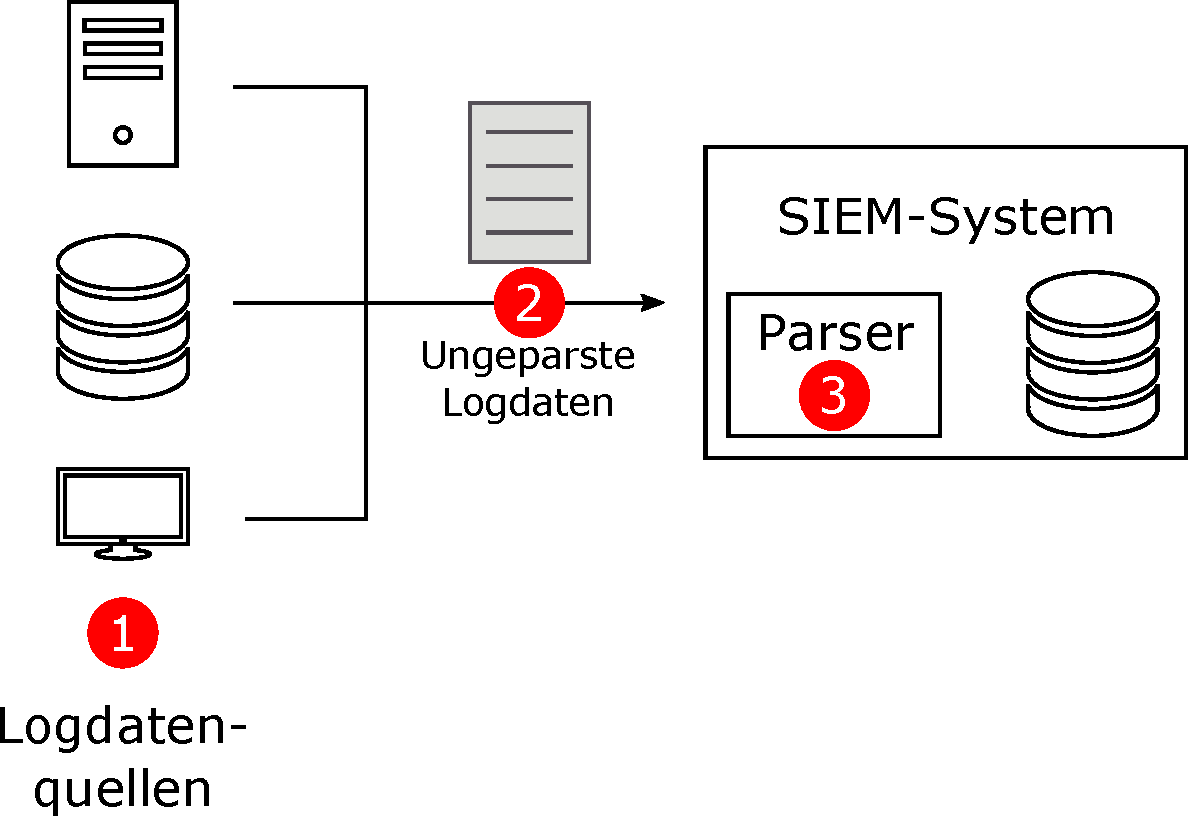
\includegraphics[width=0.5\textwidth]{dia/siem_data_access_point.pdf}
    \caption{Mögliche Eingriffspunkte in den Datenfluss eines SIEM-Systems.}
    \label{fig:siem_data_access_point}
\end{figure}

\begin{enumerate}

\item \textbf{In der Quelle der Logdaten}\\
  Bei diesem Ansatz werden die Daten bereits pseudonymisiert, bevor sie die Datenquelle verlassen. Dieser Ansatz sorgt dafür, dass die Daten bereits pseudonymisiert auf der Übertragungsstrecke und im SIEM-System vorliegen. Es ist kein mehrfaches Parsen der Daten notwendig und der Ansatz ist unabhängig vom verwendeten SIEM-System zu realisieren. Auf der anderen Seite macht der Ansatz die universelle Veränderung jeder Datenquelle notwendig. Dies kann bei Datenquellen, die auf ähnlichen gut erweiterbaren Plattformen beruhen, relativ einfach umzusetzen sein. Beispielsweise könnte die im nächsten Ansatz vorgestellte Proxy-Komponente lokal auf der Datenquelle eingesetzt werden. Schwierigkeiten würde dieser Ansatz hingegen bei Datenquellen bereithalten, die beispielsweise aus Gründen abgespeckter zugrundeliegender Betriebssysteme oder geringer Rechenleistung nur schwer erweiterbar sind. Außerdem würde er in vielen Fällen die Kooperation des Herstellers voraussetzen, wenn es sich um nicht quelloffene \glqq{}Box\grqq{}-Lösungen handelt.

\item \textbf{Proxy-basierter Ansatz}\\
  Dieser Ansatz pseudonymisiert die Daten vor dem ersten Kontakt mit dem SIEM-System, indem Datenquellen ihre Logdaten an einen Proxy senden, der die Daten pseudonymisiert und erst anschließend an das SIEM-System weiterreicht. Hierdurch wird erreicht, dass die Daten zu keiner Zeit nicht-pseudonymisiert in dem SIEM-System vorliegen. Außerdem ist er unabhängig von Datenquellen und SIEM-System und erfordert keinen direkten Eingriff in diese (abgesehen von geringen Konfigurationsanpassungen). Ein Nachteil dieser Lösung ist, dass sie das Parsen und Neuzusammensetzen der Logdaten im Proxy zusätzlich zu deren anschließender Behandlung im SIEM-System erfordert. Außerdem müssen für verschiedene Arten der Logdatenübermittlung (Protokolle wie syslog oder SNMP) unterschiedliche Proxys entwickelt werden.

\item \textbf{Patchen des SIEM-Systems}\\
  Die letzte Möglichkeit ist das Verändern des SIEM-Systems selbst. Hierzu wird in die Logdaten parsende Komponente eingegriffen, um vor, während oder nach diesem Vorgang die Logdaten zu pseudonymisieren. Dieser Ansatz erfordert kein mehrfaches Bearbeiten von Logdaten wie in dem Proxy-basierten Ansatz. Auf der anderen Seite ist er abhängig vom eingesetzten SIEM-System und erfordert seine Veränderung. Zusätzlich liegen die Daten erst einmal in nicht veränderter Form im SIEM-System vor, was die in Abschnitt \ref{subsec_impl_requirements_ossimintegration} erwähnten Nachteile mit sich bringt.

\end{enumerate}

Aus datenschutztechnischer Sicht ist eine frühestmögliche Pseudonymisierung zu bevorzugen, wie sie auch in \cite{schwartmann2017} empfohlen wird: 
\glqq{}Die Pseudonymisierung ist im Verarbeitungsprozess so früh wie möglich durchzuführen.\grqq{}
Daher wäre eine Pseudonymisierung bereits in der Datenquelle der Optimalfall. Demgegenüber stehen jedoch die erwähnten Nachteile des ersten Ansatzes im Bezug auf die Umsetzbarkeit, da hierzu jede mögliche Quelle von Logdaten universell verändert werden müsste. Eine erst im SIEM-System stattfindende Pseudonymisierung bringt jedoch die beschriebenen Risiken im Bezug auf das Vorliegen des pseudonymisierten Daten im Originalformat mit.

Dies ließ die Entscheidung auf den Proxy-basierten Ansatz fallen. Dass die Lösung außerdem noch keine Anpassungen an dem SIEM-System selbst erfordert, wiegt den Nachteil des zusätzlichen Parsens und wieder Zusammensetzens der Lognachricht bei Weitem auf.
\todo{Auch auf Angreifermodell beziehen?}

\subsection{Architektur}

%- Wie deckt dieser Ansatz die Anforderungen ab?
%  - Einbindung OSSIM
%  - Pseudonymisierung
%  - Schwellwert
%  - Benutzerinteraktion
%  - Erweiterbarkeit Datenquellen
%  - Erweiterbarkeit Datenschutztechniken

Ausgehend von diesen Überlegungen wurde ein System entworfen, dass die Anforderungen aus Abschnitt \ref{sec_impl_requirements} erfüllt und an der beschriebenen Stelle in den Datenfluss eingreift. 

%\todo{Hier erweitern: Warum verteilte Lsg (ProxyPlugin - Service):
%  - Erweiterbarkeit (Mehrere Proxy-Server mit verschiedenen Protokollen, evtl. auch direkt Client-seitig, ...) => Absicherung einer Komponente, die jedoch auch nicht alles erfährt
%  - Trennung Verarbeitung und Speicherung (Kompr. DB -> Pseudonyme bleiben verdeckt, Kompr. Proxy -> bisherige Daten und Daten evtl. anderer Proxys bleiben abgesichert)
%}

Bei dem Entwurf handelt es sich um ein verteiltes System, bei der die Verarbeitung der Logdaten und die Speicherung der Pseudonymzuordnung an unterschiedlichen Stellen geschieht. Hierfür sprechen verschiedene Gründe. Die Kompromittierung der speichernden Komponente schützt die erstellten Pseudonyme vor Aufdeckung durch die Verschlüsselung der Datensätze mit einem kryptographischen Schwellwertschema. Die Kompromittierung der verarbeitenden Komponente lässt zwar eine Verknüpfung neu erstellter Pseudonyme mit eintreffenden Daten zu, sorgt aber nicht für eine Aufdeckung bereits erstellter Pseudonyme, da diese in der anderen Komponente vorliegen. Weiterhin sorgt dieser Ansatz auch für eine zusätzliche Erweiterbarkeit des Systems. Eine speichernde Komponente kann so als Datenspeicher für mehrere verarbeitende Komponenten agieren, was beispielsweise die Erweiterung um zusätzliche Protokolle (vgl. Abschnitt \ref{sec_impl_integration_into_ossim}) oder Pseudonyme über verschiedene Datenarten (vgl. Abschnitt \ref{sec_state_se_furtherpossibilities}) ermöglicht.
Einen Überblick über den Entwurf bietet Abbildung \ref{fig:high__level_architecture}. Die verschiedenen Komponenten des Systems werden im Folgenden näher beschrieben.

\begin{figure}[]
    \centering
        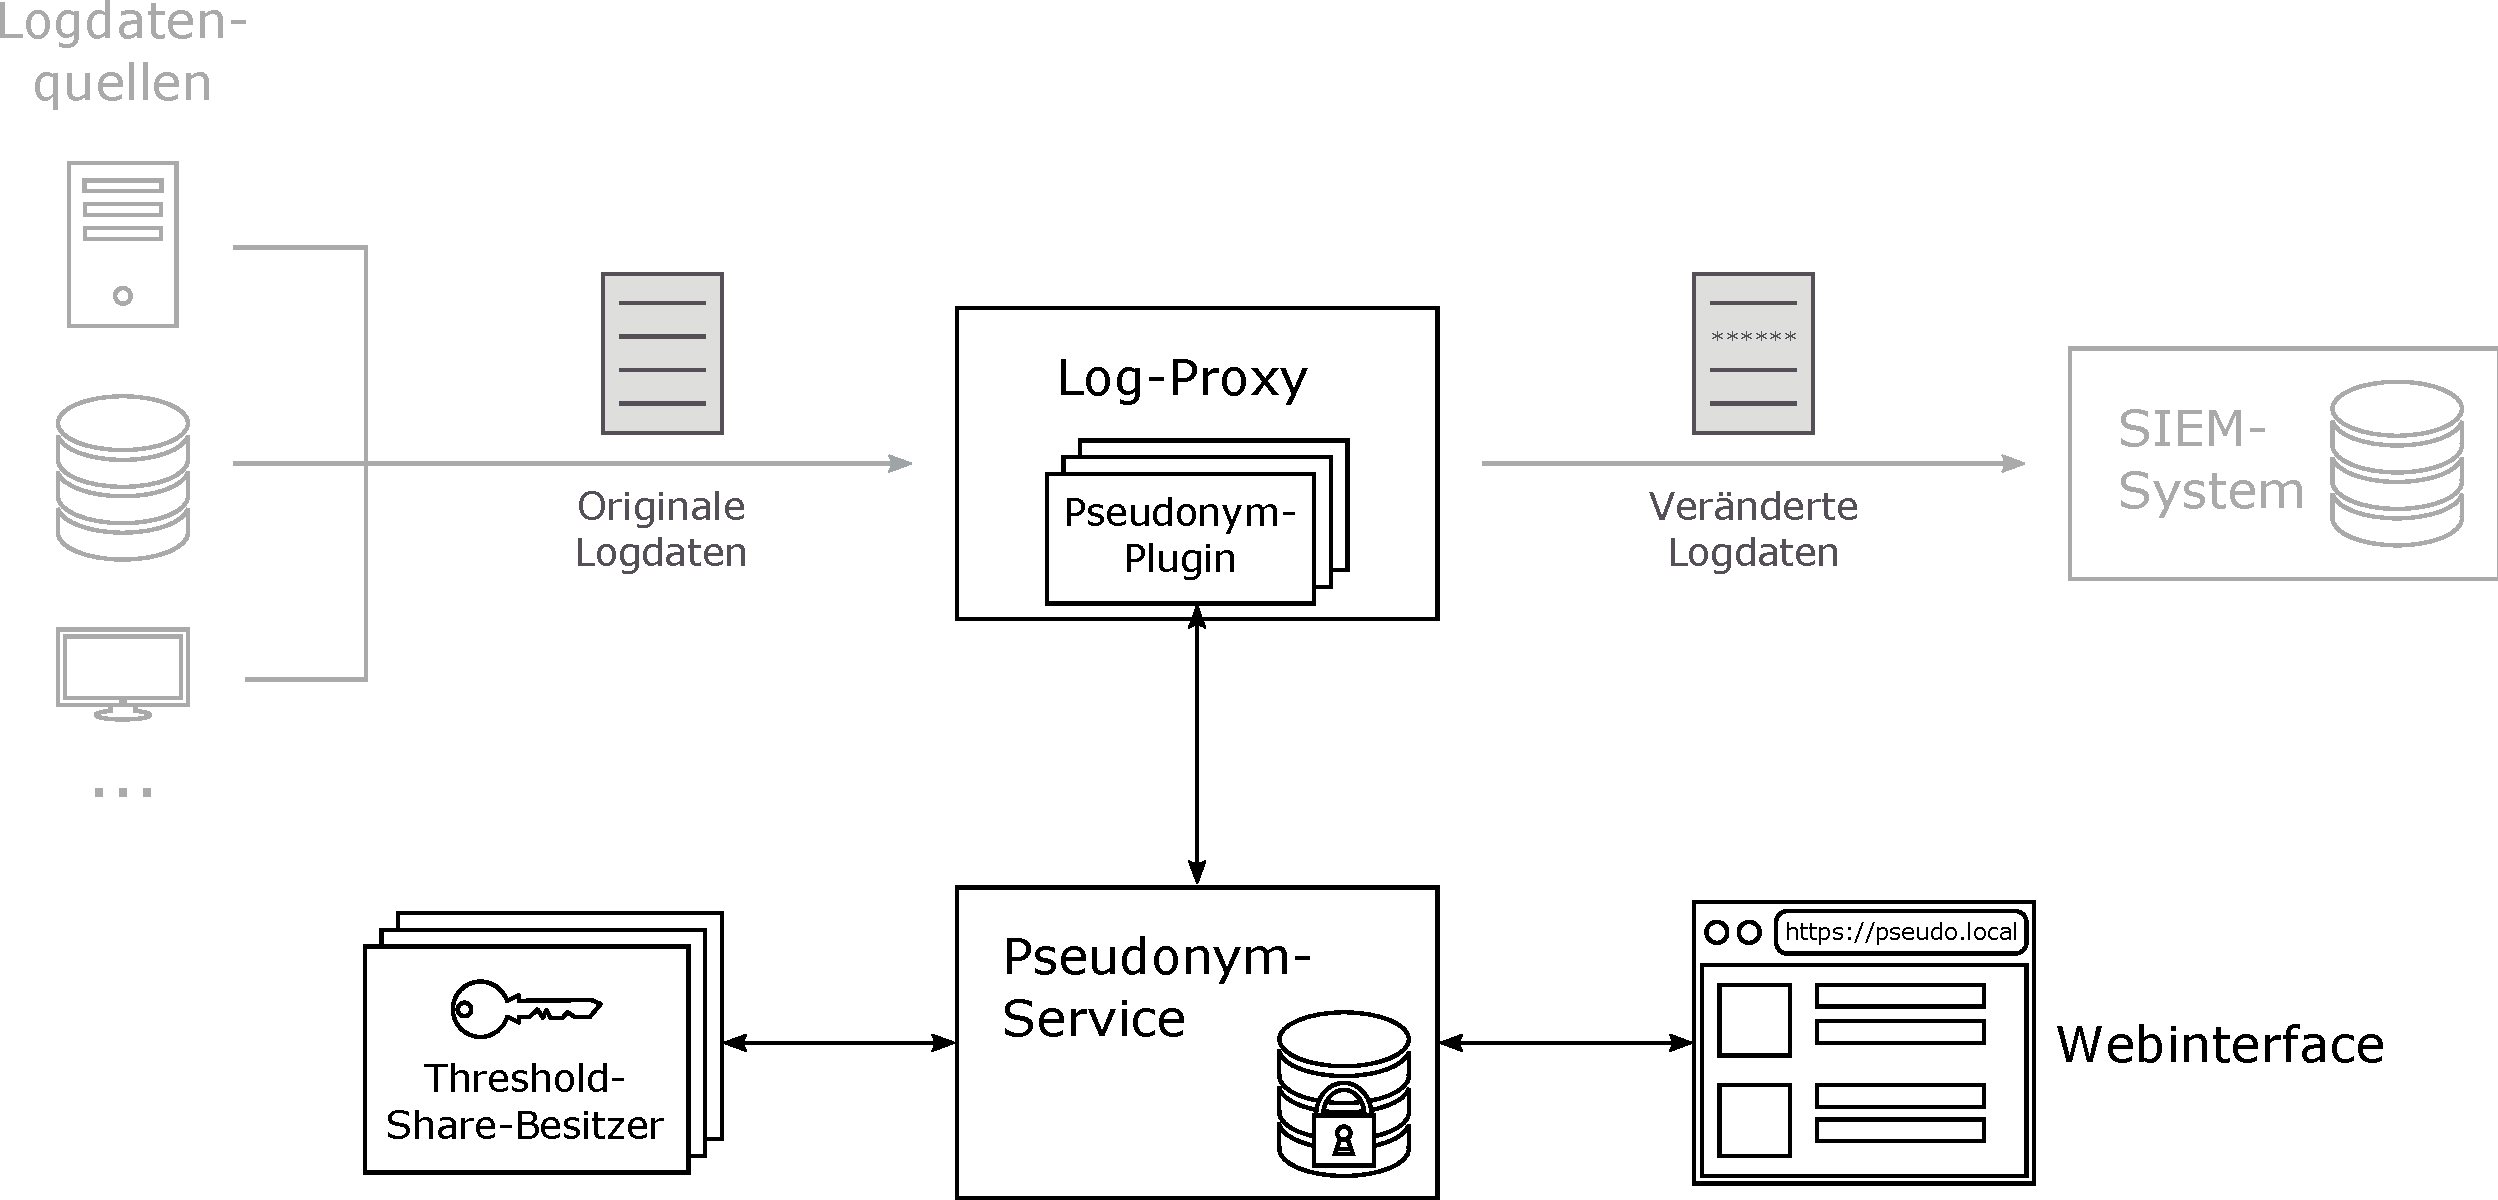
\includegraphics[width=0.9\textwidth]{dia/high_level_architecture.pdf}
    \caption{Ein Überblick über die entworfene Architektur.}
    \label{fig:high__level_architecture}
\end{figure}

Die erste Komponente ist der \textbf{Log-Proxy}, der die Daten entgegennimmt, verändert und anschließend an das SIEM-System weiterleitet. Das Verändern der Daten kann mit verschiedenen Plugins geschehen, so dass neben der umzusetzenden Pseudonymisierung auch weitere Datenschutztechniken eingesetzt werden können, was die geforderte Erweiterbarkeit aus Abschnitt \ref{subsec_impl_requirements_plugins} ermöglicht. Der Proxy leistet die Behandlung von Logdaten aus verschiedenen Quellen wie in Abschnitt \ref{subsec_impl_requirements_differentsources} beschrieben. Das für diese Art des Dateneingriffs erforderliche Parsen und Wiederzusammensetzen der Daten muss hier Datenquellen-abhängig konfigurierbar geschehen.

Ein in dem Proxy enhaltenes Plugin ist für die Pseudonymisierung von Daten zuständig und kommuniziert dazu mit einer externen Komponente -- dem Pseudonym-Service. Die Kommunikation mit dem Proxy erfolgt über einen Webservice-basierten Ansatz. Das Plugin kann für eingehende Daten ein Pseudonym anfordern und dieses anschließend in der Logdatenverarbeitung verwenden.

Der \textbf{Pseudonym-Service} erfüllt zwei Aufgaben: das Speichern und Verwalten der Pseudonyme sowie die Integrierung des kryptographischen Schwellwertschemas. Initial muss die Schlüsselgenerierung des Schwellwertschemas durch den Service geleistet werden. Dies kann wie bereits im vorhergehenden Abschnitt beschrieben zentral oder verteilt geschehen.\\
Es können während des Betriebs neue Pseudonyme angelegt und zusammen mit ihrem durch das Schwellwertschema verschlüsselten Datum abgelegt werden. Sie werden durch geeignete Maßnahmen durchsuchbar gehalten, um für ein Datum überprüfen zu können, ob bereits ein Pseudonym vergeben wurde. 
Über ein Webinterface kann ein berechtiger Benutzer die Aufdeckung eines bestimmten Pseudonyms fordern und den Status seiner Forderung bzw. im Erfolgsfall das aufgedeckte Datum betrachten. Dieses Datum wird durch das Kombinieren der partiellen Entschlüsselungen erhalten, die von den entsprechenden \textit{Share}-Besitzern berechnet werden. Weiterhin kann über dieses Webinterface auch die initiale Konfiguration des Systems im Bezug auf Eigenschaften des Pseudonymisierung und des kryptographischen Schwellwertschemas vorgenommen werden.

Benutzer, die zuständig für die Bewertung von Anfragen zur Aufdeckung eines Pseudonyms sind, erhalten die Möglichkeit zur Interaktion mit dem System über eine \textbf{Client-Anwendung}, für die der Pseudonym-Service ebenfalls als Webservice agiert. Diese Anwendung verwaltet den \textit{Share} des Benutzers für das kryptographische Schwellwertschema und kann nach der Bestätigung des Benutzers zu der Aufdeckung eines Pseudonyms die partielle Entschlüsselung eines Datensatzes erstellen und an den Pseudonym-Service senden.


\section{Zugrundeliegendes Angreifermodell}

\label{subsec_impl_requirements_attackermodel}

% Das Angreifermodell definiert die	maximal	berücksichtigte	Stärke eines Angreifers, gegen den ein	Schutzmechanismus	gerade noch wirkt.	
%Es beschreibt:
%–  Rollen des Angreifers (Außenstehender, Benutzer, Betreiber, Wartungsdienst, Produzent, Entwerfer …), auch kombiniert 
%–  Verbreitung des Angreifers (Stellen im System, an denen der Angreifer Informationen gewinnen oder Systemzustände verändern kann) 
%–  Verhalten des Angreifers 
%  •  passiv / aktiv,  beobachtend / verändernd 
%–  Rechenkapazität des Angreifers 
%  •  unbeschränkt: informationstheoretisch 
%  •  beschränkt: komplexitätstheoretisch 

Im Kontext dieser Arbeit, die sich mit der datenschutzfreundlichen Speicherung von Überwachungsdaten beschäftigt, muss zuerst folgende Vorüberlegung getroffen werden: Logdaten erreichen das verwendete SIEM-System abhängig von den verwendeten Protokollen im allgemeinen nicht-pseudonymisiert und oftmals weder verschlüsselt noch mit geschützer Integrität über das Netzwerk. \todo{Angriffsmöglichkeiten erläutern: Mitschneiden aller Daten und damit  Aufdecken von Pseudonymen, ...}
Diese Angriffsmöglichkeiten zu verhindern, ist ausdrücklich kein Ziel dieser Arbeit. Daher bezieht sich das Angreifermodell auf die Bearbeitung und Speicherung von Logdaten, erst sobald sie das zu entwickelnde System erreichen, jedoch nicht vorher.

Das Ziel des Systems bezogen auf seine Sicherheit lässt sich folgendermaßen definieren: Das Pseudonym eines Nutzers erlaubt (ohne Anwendung von Hintergrundwissen) keinen Rückschluss auf die Identität eines Nutzers. Erst die Kollaboration berechtigter Akteure ermöglicht das Aufdecken eines Pseudonyms.\todo{? außerdem erweitern um aktive Angreifer?}

Ein Angreifermodell beschreibt die maximale Stärke eines Angreifers im Bezug auf verschiedene Faktoren, gegen die ein System abgesichert ist. Enthalten sind die Rolle eines Angreifers, seine Verbreitung im System, aktives oder passives Verhalten und die Rechenkapazität, die der Angreifer zum Überwinden der eingesetzten Schutzmaßnahmen aufbringen kann. Es bildet die Basis für alle Folgeüberlegungen im Bezug auf die Sicherheit des zu entwickelnden Systems.

Für das Angreifermodell werden folgende Annahmen getroffen: Bei dem Angreifer kann es sich um einen Außenstehenden, um einen Berechtigten mit Zugriff auf das SIEM-System oder sogar um einen Administrator mit physischem Zugriff auf Rechner im Netz handeln. Wie bereits beschrieben, wird die ungesicherte Übertragung nicht-pseudonymisierter Daten zu dem System nicht betrachtet. Insofern wird von einem Angreifer ausgegangen, der erst Zugriff auf das zu entwickelnde System oder das SIEM-System beseitzt oder erlangt. Das zu entwickelnde System soll in der Lage sein, sich auch gegen aktive Angreifer zur Wehr zu setzen. \todo{Denial of Service etc?}
Bezogen auf die verfügbare Rechenleistung des Angreifers sollen verbreitete und nach heutigem Wissensstand für sicher befundene kryptographische Algorithmen als nicht mit vertretbarem Aufwand zu brechen angesehen werden. Es handelt sich daher um die Annahme von komplexitätstheoretischer Sicherheit.
